%%%%%%% Lecture Notes Style for Concrete Mathematics %%%%%%%%%%%%%
%%%%%%% Taught by Patrick White, TJHSST %%%%%%%%%%%%%%%%%%%%%%%%%%

\documentclass[11pt,twosided]{article}
%%%%%%%%%%%%%%%%%%%%%%%%%%%%%%%%%%%%%%%%%%%%%%%%%%%%%%%
%%%% HEADER FILE for CONCRETE MATH LECTURE NOTES %%%%%%
%%%%%%%%%%%%%%%%%%%%%%%%%%%%%%%%%%%%%%%%%%%%%%%%%%%%%%%

%%%%%%%%%%%%%%%%%%%%%%%%%%%%%%%%%%%%%%%%%%%%%%%%%%%%%%%%%%%%%%%%%%%
%% This file is included at the top of every lecture notes file %%%
%% It should ONLY be changed by the instructor %%
%%%%%%%%%%%%%%%%%%%%%%%%%%%%%%%%%%%%%%%%%%%%%%%%%%%%%%%%%%%%%%%%%%%

%%%%%%%%%%%%%%%%%%%%%% package inclusions %%%%%%%%%%%%%%%%%%%%
%\usepackage[
%top=2cm,
%bottom=2cm,
%left=3cm,
%right=2cm,
%headheight=17pt, % as per the warning by fancyhdr
%includehead,includefoot,
%heightrounded, % to avoid spurious underfull messages
%]{geometry} 


\usepackage{amsmath,amssymb,amsfonts}
\usepackage{longtable}
\usepackage{mathtools}
\usepackage{amsthm}
\usepackage{enumerate}
\usepackage{fancyhdr}
\pagestyle{fancy}


%%%%%%%%%%%%%%% theorem style definitions %%%%%%%%%%%%%%%%%%%%%%
\newtheorem{theorem}{Theorem}[section]
%\newtheorem{corollary}{Corollary}[theorem]
%\newtheorem{lemma}[theorem]{Lemma}
\newtheorem*{remark}{Remark}
%\newtheorem{example}{Example}[section]
\newtheorem*{definition}{Definition}


%%%%%%%%%%%%%%%% custom function definitions %%%%%%%%%%%%%%%%%%%%%%%%%
%%%%%%%%%%% as class progresses, this section may be enhanced %%%%%%%%

\def\multiset#1#2{\ensuremath{\left(\kern-.3em\left(\genfrac{}{}{0pt}{}{#1}{#2}\right)
		\kern-.3em\right)}} %%% multiset notation
\newcommand\rf[2]{{#1}^{\overline{#2}}} %%%% rising factorial \rf{x}{m}
\newcommand\ff[2]{{#1}^{\underline{#2}}} %%%%% falling factorial \ff{x}{m}
\newcommand{\Perm}[2]{{}^{#1}\!P_{#2}} % permutation
\newcommand{\half}{\ensuremath{\frac{1}{2}}}
\newcommand{\braces}[1]{\left\{#1\right\}}
\newcommand{\set}[1]{\braces{#1}}
\newcommand{\snb}[2]{\ensuremath{\left(\kern-.3em\left(\genfrac{}{}{0pt}{}{#1}{#2}\right)\kern-.3em\right)}}
\newcommand{\fallingfactorial}[1]{^{\underline{#1}}}
\newcommand{\fallfac}[2]{{#1}^{\underline{#2}}}
\newcommand{\stirlingone}[2]{\genfrac[]{0pt}{1}{#1}{#2}}
\newcommand{\stiri}[2]{\stirlingone{#1}{#2}}
\newcommand{\dstirlingone}[2]{\genfrac[]{0pt}{0}{#1}{#2}}
\newcommand{\dstiri}[2]{\dstirlingone{#1}{#2}}
\newcommand{\stirlingtwo}[2]{\genfrac\{\}{0pt}{1}{#1}{#2}}
\newcommand{\stirii}[2]{\stirlingtwo{#1}{#2}}
\newcommand{\dstirlingtwo}[2]{\genfrac\{\}{0pt}{0}{#1}{#2}}
\newcommand{\dstirii}[2]{\dstirlingtwo{#1}{#2}}
\newcommand{\ol}[1]{\overline{#1}}
%%%%%%%
% book stuff
%%%%%%%%%

\usepackage[twoside,outer=1.5in,inner=2in,bottom=1.5in,top=1.5in,marginpar=2in]{geometry} 
\usepackage{scrextend}
\usepackage{palatino}
\usepackage{multicol}
\usepackage{float}
\usepackage[hidelinks]{hyperref}
\usepackage[nameinlink, capitalise, noabbrev]{cleveref}
%\usepackage{background}
\usepackage{graphicx}
\usepackage{listliketab}

\usepackage{lipsum}
\usepackage{caption}
\usepackage{marginnote}

\reversemarginpar


\usepackage[dvipsnames]{xcolor}
\usepackage{amsthm}
\usepackage{shadethm}

\setlength{\parindent}{0pt}

\newcommand*\Note{%
	\marginnote[\textcolor{blue}{\raggedright{\LARGE ?}\ Note }]{}%
}
\newcommand*\Warn{%
	\marginnote[\textcolor{red}{\raggedright{\LARGE !}\ Warning }]{}%
}
\reversemarginpar

\newcommand{\N}{\mathbb{N}}
\newcommand{\Z}{\mathbb{Z}}
\newcommand{\I}{\mathbb{I}}
\newcommand{\R}{\mathbb{R}}
\newcommand{\Q}{\mathbb{Q}}
\renewcommand{\qed}{\hfill$\blacksquare$}
\let\newproof\proof
\renewenvironment{proof}{\begin{addmargin}[1em]{0em}\begin{newproof}}{\end{newproof}\end{addmargin}\qed}
% \newcommand{\expl}[1]{\text{\hfill[#1]}$}


\newenvironment{lemma}[2][Lemma]{\begin{trivlist}
		\item[\hskip \labelsep {\bfseries #1}\hskip \labelsep {\bfseries #2.}]}{\end{trivlist}}
\newenvironment{problem}[2][Problem]{\begin{trivlist}
		\item[\hskip \labelsep {\bfseries #1}\hskip \labelsep {\bfseries #2.}]}{\end{trivlist}}
\newenvironment{example}[2][Example]{\begin{trivlist}
		\item[\hskip \labelsep {\bfseries #1}\hskip \labelsep{\bfseries #2.}]}{\end{trivlist}}
\newenvironment{solution}{{\noindent \bfseries Solution\hskip 2ex}}{\qed}
\newenvironment{exercise}[2][Exercise]{\begin{trivlist}
		\item[\hskip \labelsep {\bfseries #1}\hskip \labelsep {\bfseries #2.}]}{\end{trivlist}}
\newenvironment{reflection}[2][Reflection]{\begin{trivlist}
		\item[\hskip \labelsep {\bfseries #1}\hskip \labelsep {\bfseries #2.}]}{\end{trivlist}}
\newenvironment{proposition}[2][Proposition]{\begin{trivlist}
		\item[\hskip \labelsep {\bfseries #1}\hskip \labelsep {\bfseries #2.}]}{\end{trivlist}}
\newenvironment{corollary}[2][Corollary]{\begin{trivlist}
		\item[\hskip \labelsep {\bfseries #1}\hskip \labelsep {\bfseries #2.}]}{\end{trivlist}}

%%%% add package inclusions here, if any
\usepackage{graphicx}
\graphicspath{ {images12/} }
\usepackage{float}
%%%%% Define your custom functions and macros here, if any
\newcommand{\fallingfactorial}[1]{%
	^{\underline{#1}}%
}
%%%%%%%%%%%%%%%%%%%% Define the variables below %%%%%%%%%%%%%%%%%%%%%%%%%%%%%%
\def\titlestring{Three Counting Problems}
\def\scribestring{Connor Mooney}
\def\datestring{28 February 2019}


%%%%%%%%%%%%%%%%%%% Page Headers -- Do Not Change %%%%%%%%%%%%%%%%%%%%%%%%%%%
\lhead{\titlestring}
\rhead{Page \thepage}
\cfoot{Concrete Math -- White -- TJHSST}
\renewcommand{\headrulewidth}{0.4pt}
\renewcommand{\footrulewidth}{0.4pt}

%%%%%%%%%%%%%%%%% Begin the document %%%%%%%%%%%%%%%%%%%%%%%%%
\begin{document}
\thispagestyle{plain}  %% no headers on this page

%%%% Do not change these lines %%%%%
\noindent
{\LARGE \textbf{\titlestring}}\\\\
%
{\Large Scribe: \scribestring}\\ \\
{\textbf{Date}: \datestring}


%%%%%%%%%%%%%%%%%%%%%%%%%% YOUR CONTENT GOES HERE %%%%%%%%%%%%%%%%%%%%%%%%%%
\noindent

\section{Trapezoid Problem}
\begin{problem}
	1 We have $n$ rows of triangles as shown below. How many parallelograms can be formed in this figure?
\end{problem}
\begin{figure}[h]
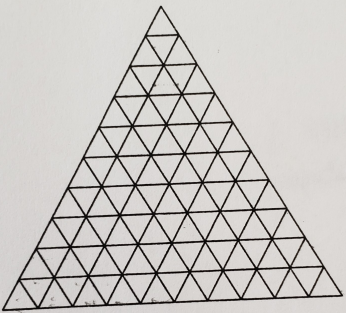
\includegraphics[scale=0.1]{TRIANGLE22.jpg}
\centering
\end{figure}
\begin{solution}
There can be three orientations of parallelograms, shown below, which by symmetry must have the same number of parallelograms. Thus, we can count one and multiply that number by three.
\begin{figure}[H]
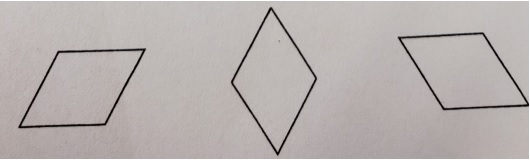
\includegraphics[scale=0.1]{TRIANGLE23.jpg}
\centering
\end{figure}
We can observe that a parallelograms has four lines that can be extended out. If we extend them out to one layer lower than the triangle, we can notice that the lines intersect with the bottom layer to find four points. Each one of the parallelograms corresponds to a unique selection of the four points, and vice versa.
\begin{figure}[H]
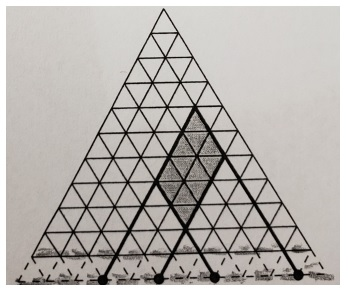
\includegraphics[scale=0.1]{TRIANGLE24.jpg}
\centering
\end{figure}
Thus, for each of the $n+2$ points on the level below the last one, we can choose four of them to get a unique parallelogram. Thus, in conclusion, the solution is \[3\cdot{n+2 \choose 4}\]
\end{solution}
\section{Hat Problem}
\begin{problem}
	2 n mathematicians walk into a bar. They each remove their hat and toss it in a pile as they arrive. Several hours later, they leave one by one, grabbing a hat at random to face the brutal March wind. What is the probability that none of the mathematicians receive their own hat?
\end{problem}
\begin{solution}
	This problem is equivalent to finding the number of \textbf{Derangement} of a set of size n, up to a factor of $n!$. The derangement number is notated as $D_n,$ or $!n.$
	\newline
	We can approach this by counting the number of ways to get the desired outcome via complementary counting, and then to divide it through by the total number of arrangements to get the probability, as each configuration is equally likely. First, to count the number of ways in total that there can be reordered. This is just n!. However, in this, we have counted the number of ways that at least $0$ mathematicians receive their hat. Next, we must subtract out the cases that have at least $1$ mathematician getting back his or her hat. We can count this by choosing which mathematician gets his or her hat back, and then ordering the rest. Thus, the term is ${n\choose1}\left(n-1\right)!.$ However, this overcounts those configurations for which more than one mathematician receives their hat back; we can fix this problem by using the principle of inclusion/exclusion, to get that the total number of derangements is \[n!-{n\choose1}\left(n-1\right)!+{n\choose2}\left(n-2\right)!+\cdots+(-1)^n{n\choose n}\left(n-n\right)!.\]
	This approaches $\frac{n!}{e}$ for sufficiently large $n$, as $e^x=1+x+x^2/2!+\cdots.$ Thus, by dividing the nth derangement number by $n!,$ we get the probability to be \[1-\frac{1}{1!}+\frac{1}{2!}+\cdots+\frac{(-1)^n}{n!}\approx e^{-1}\] for sufficiently large n.
\end{solution}
\section{"Coupon Collector"-esqe Problem}
\begin{problem}
	3 You have a bag containing $x$ numbered marbles. Draw $n$ marbles with replacement, where $n\leq x$. What is the probability that you drew exactly $k$ distinct marbles?
\end{problem}
\begin{solution}
To solve this, we can consider sequences of draws. First, we must determine the total number of "events" or valid sequences. There are $x^n$ such sequences. Next, we must pick $k$ of the $x$ distinct marbles to be seen, introducing a factor of ${x\choose k}.$ Next, we must partition the sequence of $n$ draws into $k$ subsets, each subset representing the draws that got one distinct value of the marble, introducing a factor of $S(n,k)$. And finally, we must assign each marble to a subset, introducing a factor of $k!.$ Thus, the probability is \[\frac{k!{x \choose n}S(n,k)}{x^n}.\]
\begin{example}
		If there are $10$ distinct marbles, we Draw $6$, and see $3$, one possible outcome is, if the number $j$ represent the $jth$ draw, \[C:\{1,4\},A:\{2,3,5\},B:\{6\}\]
		
\end{example}
Simplifying the probability a small amount, we get it to be \[\frac{x\fallingfactorial{k}S(n,k)}{x^n}.\]
This also turns out to be a way to prove that $x^n=\sum_{k=1}^{n}x\fallingfactorial{k}S(n,k),$ as the sum of the probabilities of all valid outcomes must be one.
\end{solution}
\end{document}
